	\section{Fórmulas de Little}
	Hay ciertos datos que nos pueden resultar muy interesantes de obtener, como el n\'umero medio de personas en el sistema o el tiempo medio que un cliente pasa en \'el. Definimos los siguientes t\'erminos:
	\begin{itemize}
		\item $\lambda$ = ratio de entrada de clientes por unidad de tiempo
		\item$L$ = n\'umero medio de clientes en el sistema
		\item$L_q$ = n\'umero medio de clientes en la cola
		\item$L_s$ = n\'umero medio de clientes siendo servidos
		\item$W$ = tiempo medio que un cliente pasa en el sistema
		\item$W_q$ = tiempo medio que un cliente pasa en la cola
		\item$W_s$ = tiempo medio que un cliente tarda en ser servido
	\end{itemize}
\hspace{0.5cm}	En estas definiciones, siempre asumimos que estamos en el estado de equilibrio. Para la mayor\'ia de colas, podemos escribir las f\'ormulas de Little como en el siguiente teorema.
	\subsection{Teorema}
	Para cualquier sistema de colas en el que exista el estado estable, se tienen las siguientes relaciones:
	\begin{itemize}
		\item $L=\lambda W$
		\item$L_q=\lambda W_q$
		\item$L_s=\lambda W_s$
	\end{itemize}
\hspace{0.5cm}	Vamos a dar una prueba intuitiva, debido a la gran dificultad de la prueba anal\'itica. \\
\hspace{0.5cm}Consideramos un sistema de colas con pol\'itica FCFS. Supongamos una llegada arbitraria. Cuando este cliente abandone el sistema, habr\'a de media en el sistema $L$ clientes. Por otro lado, cuando este cliente se haya, las personas que queden en el sistema ser\'an aquellas que han llegado en el tiempo que el cliente ha pasado en el sistema, $W$. Como el ratio de entrada es $\lambda$, tenemos que $L=\lambda W$.\\
\hspace{0.5cm}	Es interesante saber que la prueba anal\'itica es independiente de la pol\'itica de servicio, el n\'umero de servicios, la distribuci\'on del tiempo de llegada y del tiempo de servicio, por lo que las f\'ormulas de Little nos ser\'an v\'alidas en cualquier sistema de colas en el que se pueda alcanzar el estado de equilibrio.

\section{M/M/1}
En este modelo, el tiempo entre llegada sigue una distribuci\'on exponencial (suponemos que $\lambda$ es el ratio de llegada por unidad de tiempo) y el servidor tiene tiempos de servicio exponenciales ( suponemos que el ratio de tiempo de servicio es $\mu$ ). Como ya hemos demostrado, este modelo puede ser representado como un proceso de nacimiento-muerte con los siguientes par\'ametros:
	$$\begin{array}{cc}
	\lambda_j=\lambda & (j=0,1,...)\\
	\mu_0=0 &  \\
	\mu_j=\mu &  (j=1,2,...)\\
	\end{array}$$
	
Con estos par\'ametros y sabiendo que $\pi_j=\pi_0 c_j$ tenemos que:
	\begin{center}
		$\pi_1=\pi_0\rho, \qquad \pi_2=\pi_0\rho^2, \qquad...,\qquad\pi_j=\pi_0\rho^j$
	 
	\end{center}
\hspace{0.5cm}Donde $\rho=\frac{\lambda}{\mu}$, a lo que llamaremos intensidad de tr\'afico. Como la suma de todos los estados es $1$ llegamos a:
	\begin{center}
		$$\sum_{j=0}^{\infty}\pi_j=\pi_0(1+ \rho +\rho^2+\rho^3+...)=1$$
	\end{center}
\hspace{0.5cm}Vamos a asumir que $0\leq rho<1$. Vamos a calcular $S=1+ \rho +\rho^2+\rho^3+...$. Para ello multiplicamos $S$ por $\rho$, $S\rho=\rho+\rho^2+\rho^3+...$ y hacemos $S-\rho S=1$, de donde $S=\frac{1}{1-\rho}$.\\
\hspace{0.5cm}Sustituyendo en por el valor obtenido de $S$
	\begin{center}
		$\pi_0=1-\rho$
	\end{center}
\hspace{0.5cm}Y sustituyendo en la expresi\'on que tenemos para $\pi_j$ finalmente llegamos al resultado
	\begin{center}
		$\pi_j=\rho^j(1-\rho)$
	\end{center}
\hspace{0.5cm}Hemos asumido que $0\leq\rho<1$ para hallar la expresi\'on de $\pi_j$. Si $\rho>1$ entonces se tiene que $\lambda>\mu$, y por lo tanto el sistema no alcanzar\'ia el estado de equilibrio, ya que el ritmo de entrada de clientes ser\'ia mayor que el de salida, y por lo tanto la cantidad de gente en el sistema se disparar\'ia.\\
\hspace{0.5cm}Si $\rho=1$ no se puede ver de forma tan clara que no se alcanza el estado de equilibrio, pero tendr\'iamos que $S=1+1+1+1+...$ lo cual diverge.
	\subsection{C\'alculo de $L$}
	A partir de ahora siempre asumimos que $\rho<1$, y que hemos alcanzado el estado de equilibrio. Como $\pi_j$ indica la probabilidad de que haya $j$ individuos en el sistema, el n\'umero medio de personas en el sistema vendr\'a dado por
		\begin{center}
			$$L=\sum_{j=0}^{\infty}j\pi_j=\sum_{j=0}^{\infty}j\rho^j(1-\rho)=(1-\rho)\sum_{j=0}^{\infty} j \rho^j$$
		\end{center}  
	\hspace{0.5cm}Sea $S_2=\displaystyle \sum_{j=0}^{\infty}j\rho^j=\rho+2\rho^2+3\rho^3...$\\
	\hspace{0.5cm}Al igual que antes, hacemos $\rho S_2$ y restando: $$S_2 -\rho S_2=\rho+\rho^2+\rho^3...=\frac{\rho}{1-\rho}$$
	Despejando, tenemos que $S_2=\displaystyle\frac{\rho}{(1-\rho)^2}$ y por lo tanto
		\begin{equation}
			L=(1-\rho)\frac{\rho}{(1-\rho)^2}=\frac{\rho}{1-\rho}=\frac{\lambda}{\mu-\lambda}
		\end{equation}
	
	\subsection{C\'alculo de $L_q$ y $L_s$}
	En el modelo $M/M/1$ siempre habr\'a una persona siendo servida, excepto si no hay ninguna persona en el sistema. Por lo tanto, el n\'umero medio de personas siendo servidas $L_s$, ser\'a
		\begin{center}
			$$L_s=0\pi_0+1(\pi_1+\pi_2+...)=1-\pi_0=1-(1-\rho)=\rho$$
		\end{center}
\hspace{0.5cm}	Adem\'as, todos los clientes que est\'en en el sistema o bien est\'an en la cola o bien est\'an siendo servidos, es decir, $L=L_q+L_s$. Por lo tanto
		\begin{center}
			$$L_q=L-L_s=\frac{\rho^2}{1-\rho}$$
		\end{center}
	
	\subsection{C\'alculo de los tiempos de espera}
	Usando las f\'ormulas de Little podemos calcular f\'acilmente $W,W_q$ y $W_s$
		\begin{itemize}
			\item $W=\displaystyle\frac{L}{\lambda}=\frac{1}{\mu-\lambda}$
			\item $W_q=\displaystyle\frac{L_q}{\lambda}=\frac{\lambda}{\mu(\mu-\lambda)}$
			\item$W_s=\displaystyle\frac{L_s}{\lambda}=\frac{1}{\mu}$
		\end{itemize}
	\hspace{0.5cm}Al igual que con la cantidad media de individuos, podr\'iamos haber usado que un cliente pasa su tiempo en el sistema o esperando en la cola o siendo servido, es decir, $W=W_q+W_s$. \\
	\hspace{0.5cm}Como observaci\'on, el valor de $W_s$ lo pod\'iamos deducir desde un principio, pues al ser el tiempo del servidor exponencial de par\'ametro $\mu$, su esperanza es $\displaystyle \frac{1}{\mu}$.
	
\section{M/M/1/c}
		En este modelo, a diferencia del $M/M/1$ el sistema tiene una capacidad $c$. Se comportará igual a la $M/M/1$, excepto cuando haya $c$ personas en el sistema, momento en el cual todas las nuevas llegadas no podrán entrar en el sistema, y diremos que estas se han perdido. Suponiendo tiempos entre llegada exponenciales de ratio $\lambda$ y tiempos de servicio exponenciales de ratio $\mu$, podemos modelar esta cola como un proceso de nacimiento-muerte con los siguientes par\'ametros:
		$$\begin{array}{cc}
		\lambda_j=\lambda & (j=0,1,...,c-1)\\
		\lambda_c=0 & \\
		\mu_0=0 &  \\
		\mu_j=\mu &  (j=1,2,...,c)\\
		\end{array}$$
		\hspace{0.5cm} Como $\lambda_c=0$, la probabilidad de llegar al estado $c+1$ es $0$. Por lo tanto, las ecuaciones de balance ser\'ian:
			$$\begin{array}{cc}
		\pi_0=\displaystyle\frac{1-\rho}{1-\rho^{c+1}} & \\
		\pi_j=\rho^j\pi_0 & (j=1,2,...,c)\\
		\pi_j=0 & (j=c+1,c+2,...)\\
		\end{array}$$
		\subsection{C\'alculo de $L$} A diferencia del modelo $M/M/1$, en el $M/M/1/c$ es posible que $\rho\geq1$, ya que en este caso la cantidad de clientes no se disparar\'ia ya que cuando se llegase a $c$ clientes nadie m\'as podr\'ia entrar al sistema. Para el c\'alculo de $L$ vamos a diferenciar dos posibles casos para $\rho$
		\begin{itemize}
			\item  Si $\rho=1$ tenemos que 
			$$\begin{array}{cc}
				\pi_j=\frac{1}{c+1} & (j=0,1,...,c)\\
				L=\displaystyle\sum_{k=0}^{c}k\pi_k=\frac{1}{c+1}\sum_{k=0}^{c}k=\frac{c}{2}& \\
				\end{array}$$
		
			\item Si $\rho\neq1$

					$$L=\sum_{k=0}^{c}k\frac{\rho^k (1-\rho)}{1-\rho^{c+1}}=\frac{1}{1-\rho^{c+1}}\sum_{k=0}^{c}k\rho^k (1-\rho)=\frac{1}{1-\rho^{c+1}}(\underbrace{\sum_{k=0}^{\infty}k\rho^k(1-\rho)}_{\displaystyle\frac{\rho}{1-\rho^{c+1}}}-\sum_{k=c+1}^{\infty}k\rho^k(1-\rho))$$
					$$\sum_{k=c+1}^{\infty}k\rho^k(1-\rho)=\sum_{k=c+1}^{\infty}[k-(c+1)+(c+1)]\rho^k(1-\rho)=$$
					$$\sum_{k=c+1}^{\infty}[k-(c+1)]\rho^k(1-\rho)+\sum_{k=c+1}^{\infty}(c+1)\rho^k(1-\rho)=$$
					$$\rho^{c+1}\sum_{m=0}^{\infty}m\rho^m(1-\rho)+(c+1)\rho^{c+1}\sum_{m=0}^{\infty}\rho^m(1-\rho)=\rho^{c+1}\frac{\rho}{1-\rho}+(c+1)\rho^{c+1}$$

				Entonces acabamos diciendo que 
				\begin{center}
					$L=\frac{1}{1-\rho^{c+1}}((1-\rho^{c+1})\frac{\rho}{1-\rho}-(c+1)\rho^{c+1})=\frac{\rho}{1-\rho}-\frac{(c+1)\rho^{c+1}}{1-\rho^{c+1}}$
				\end{center}
			\subsection{C\'alculo de $L_q$ y $L_s$}
			\hspace{0.5cm} Al solo haber un \'unico servidor, el c\'alculo de $L_s$ es igual que en el modelo $M/M/1$
				$$L_s=1-\pi_0$$
			Una vez tenemos $L$ y $L_s$, es muy f\'acil obtener $L_q$
				$$L_q=L-L_s=L-1+\pi_0$$
			\subsection{C\'alculo de $W$,$W_q$ y $W_s$}
			\hspace{0.5cm}En este modelo, tenemos que $\lambda$ es el n\'umero medio de personas que llegan al sistema por unidad de tiempo. Pero al tener una capacidad finita, no todas las personas que llegan entran, pues si hay $c$ personas, el siguiente cliente en "llegar" $~$ no podr\'a entrar. Por lo tanto, la cantidad media de clientes que realmente entrar\'a en el sistema ser\'a $\lambda-\lambda\pi_c=\lambda(1-\pi_c)$. Por lo tanto, usando las f\'ormulas de Little:
			\begin{itemize}
				\item $\displaystyle W=\frac{L}{\lambda(1-\pi_0}$
				\item $\displaystyle W_q=\frac{L_q}{\lambda(1-\pi_c)}$
			\end{itemize}
	\hspace{0.5cm}	Como el tiempo que tarda cada servidor es una exponencial de ratio $\mu$, tenemos que al igual que en el modelo $M/M/1$, $W_s=\frac{1}{\mu}$.
		\end{itemize}
		
		
		\begin{figure}[h]
			\centering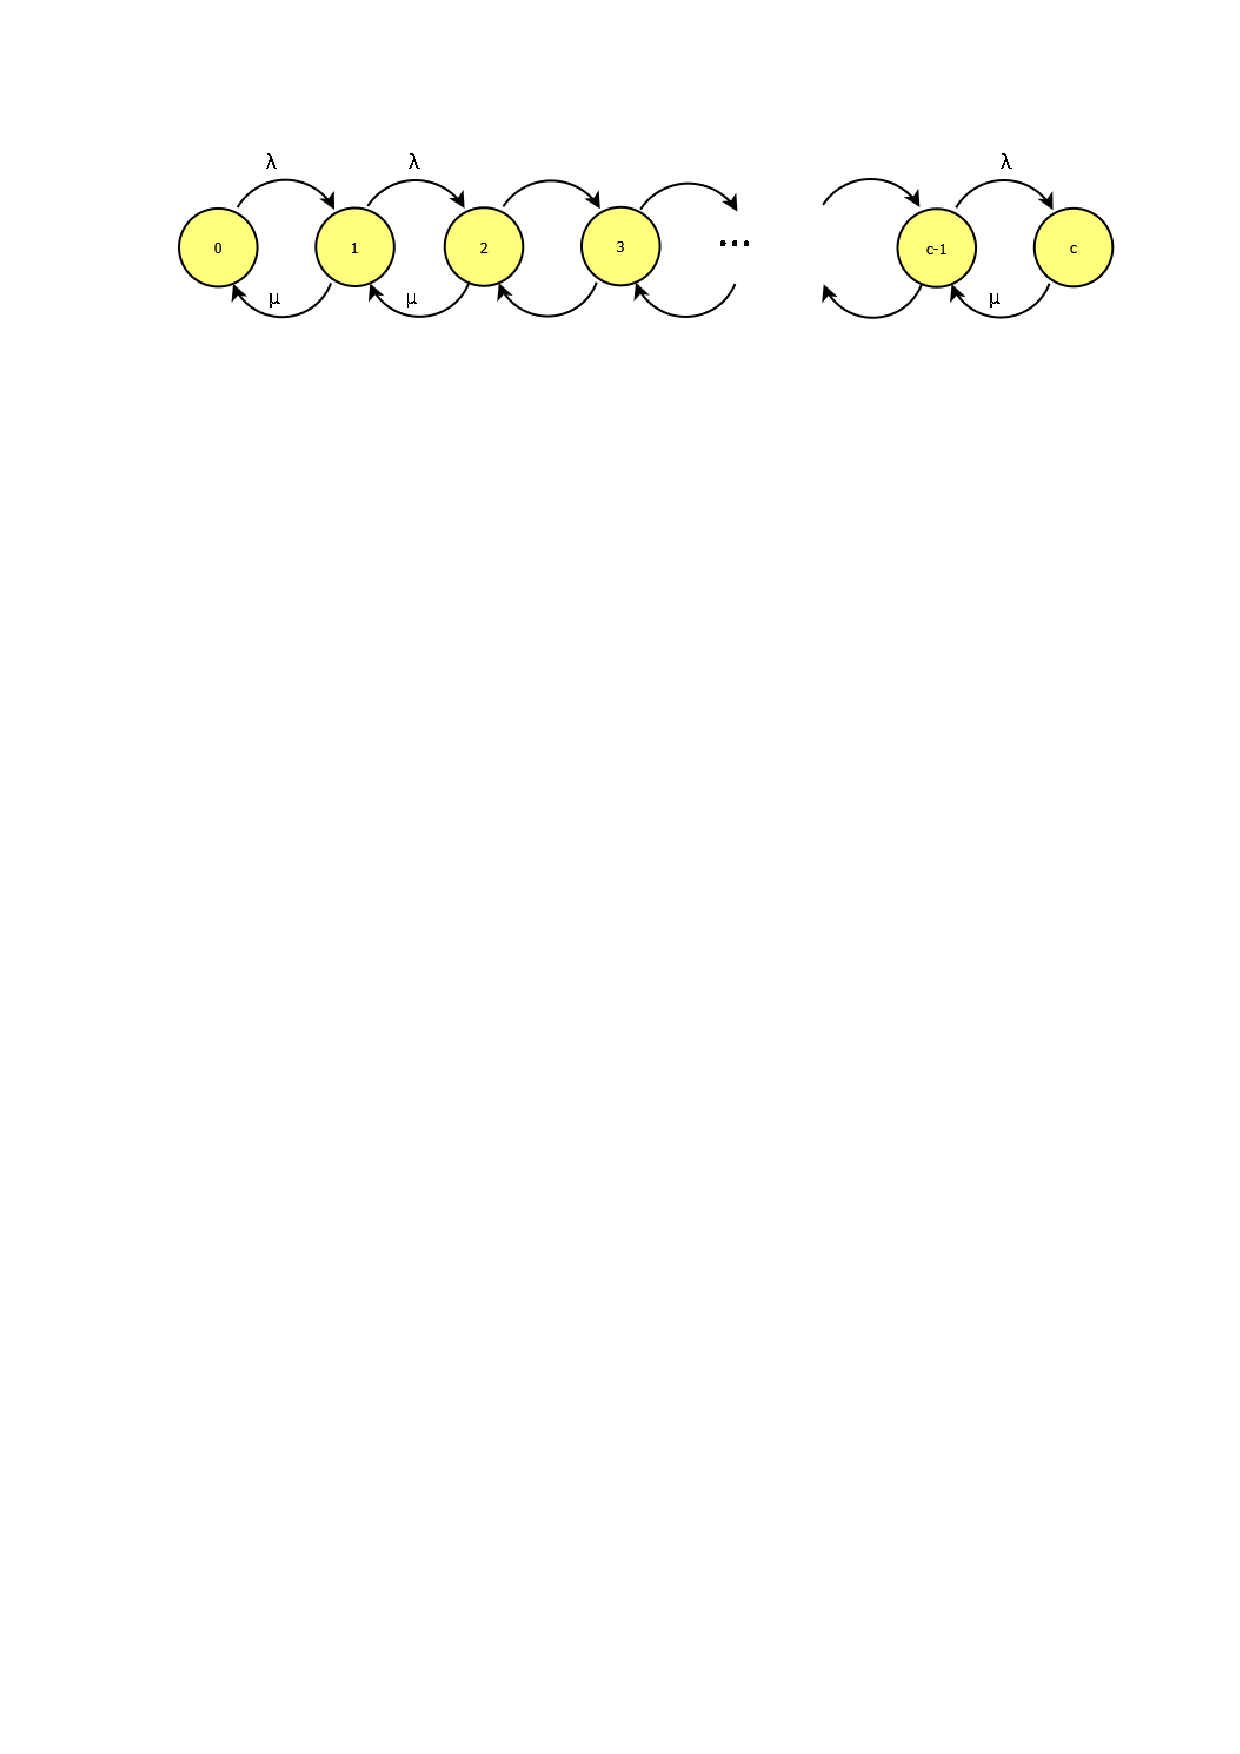
\includegraphics[trim = 10mm 220mm 10mm 25mm, clip,width=0.9\linewidth]{MMc}
		\end{figure}
		
	\section{M/M/s}
		En este modelo, la capacidad del sistema es infinita y contamos con $s$ servidores. Vamos a suponer que solo se forma una cola, y que el primero de la cola pasa al primer servidor que se quede libre. Claramente, un sistema con esta forma de espera es mucho m\'as eficiente que uno en el que se forme una cola para cada servidor, pues podr\'ia pasar que un servidor se quedase libre y nadie entrase.\\
		\hspace{0.5cm}En este modelo asumiremos que el tiempo entre llegadas es exponencial de ratio $\lambda$ y y el tiempo de servicio es exponencial de ratio $\mu$, para cada uno de los $s$ servidores.\\
		\hspace{0.5cm}Cuando en el sistema haya $j\leq s$ clientes, todos estar\'an siendo servidos. Cuando haya $j>s$, los que vayan llegando esperar\'an en la cola. Tenemos que este tipo de cola se puede modelizar como un proceso de nacimiento-muerte con los siguientes par\'ametros
		$$\begin{array}{cc}
		\lambda_j=\lambda & (j=0,1,2,...)\\
		\mu_j=j\mu & (j=1,2,...,s)\\
		\mu_j=s\mu & (j=s+1,s+2,...)\\
		\end{array}$$
		\hspace{0.5cm}Definimos $\rho=\displaystyle\frac{\lambda}{s\mu}$. Al igual que en el modelo $M/M/1$, si $\rho\geq1$, el sistema no alcanza el equilibrio pues el n\'umero de clientes se "disparar\'ia". Por lo tanto, para $\rho<1$ usando las ecuaciones de equilibrio:
		$$\begin{array}{cc}
		\pi_0=\displaystyle\frac{1}{\displaystyle \sum_{t=0}^{t=s-1}\frac{(s\rho)^t}{t!}+\frac{(s\rho)s}{s!(1-\rho)}} & \\
		\pi_j=\displaystyle\frac{(s\rho)^j\pi_0}{j!} & (j=0,1,...,s)\\
		\pi_j=\displaystyle\frac{(s\rho)^j\pi_0}{s!s^{j-s}} & (j=s+1,s+2,...)\\
		\end{array}$$
		\hspace{0.5cm} Es muy interesante saber cu\'al es la probabilidad de que todos los servidores est\'en ocupados, que viene dada por:
		$$P(j\geq s)=\sum_{k\geq s}^{}\pi_k=\sum_{k=s}^{\infty}\frac{(s\rho)^k\pi_0}{s!s^{k-s}}=\frac{s^s}{s!}\pi_0\sum_{k=s}^{\infty}\rho^k=\frac{s^s}{s!}\pi_0\rho^s\frac{1}{1-\rho}=\frac{(s\rho)^s}{s!(1-\rho)}\pi_0$$
			
		Se puede demostrar que 
		$$L_q=\frac{P(j\geq s)\rho}{1-\rho}$$
		Una vez tenemos $L_q$, usando las f\'ormulas de Little obtenemos
		$$W_q=\frac{L_q}{\lambda}=\frac{P(j\geq s)}{s\mu-\lambda}$$
		\hspace{0.5cm} Una vez que el cliente est\'a en el servidor, como este sigue una distribuci\'on exponencial, tenemos que $W_s=\frac{1}{\mu}$.\\
	    \hspace{0.5cm}	Mediante Little obtenemos $L_s=\frac{\lambda}{\mu}$. Luego
		$$L=L_q+L_s=L_q+\frac{\lambda}{\mu}$$
		De nuevo, usando Little podemos calcular $W$
		$$W=\frac{L}{\lambda}=\frac{L_q}{\lambda}+\frac{1}{\mu}$$
		
		\begin{figure}[h]
			\centering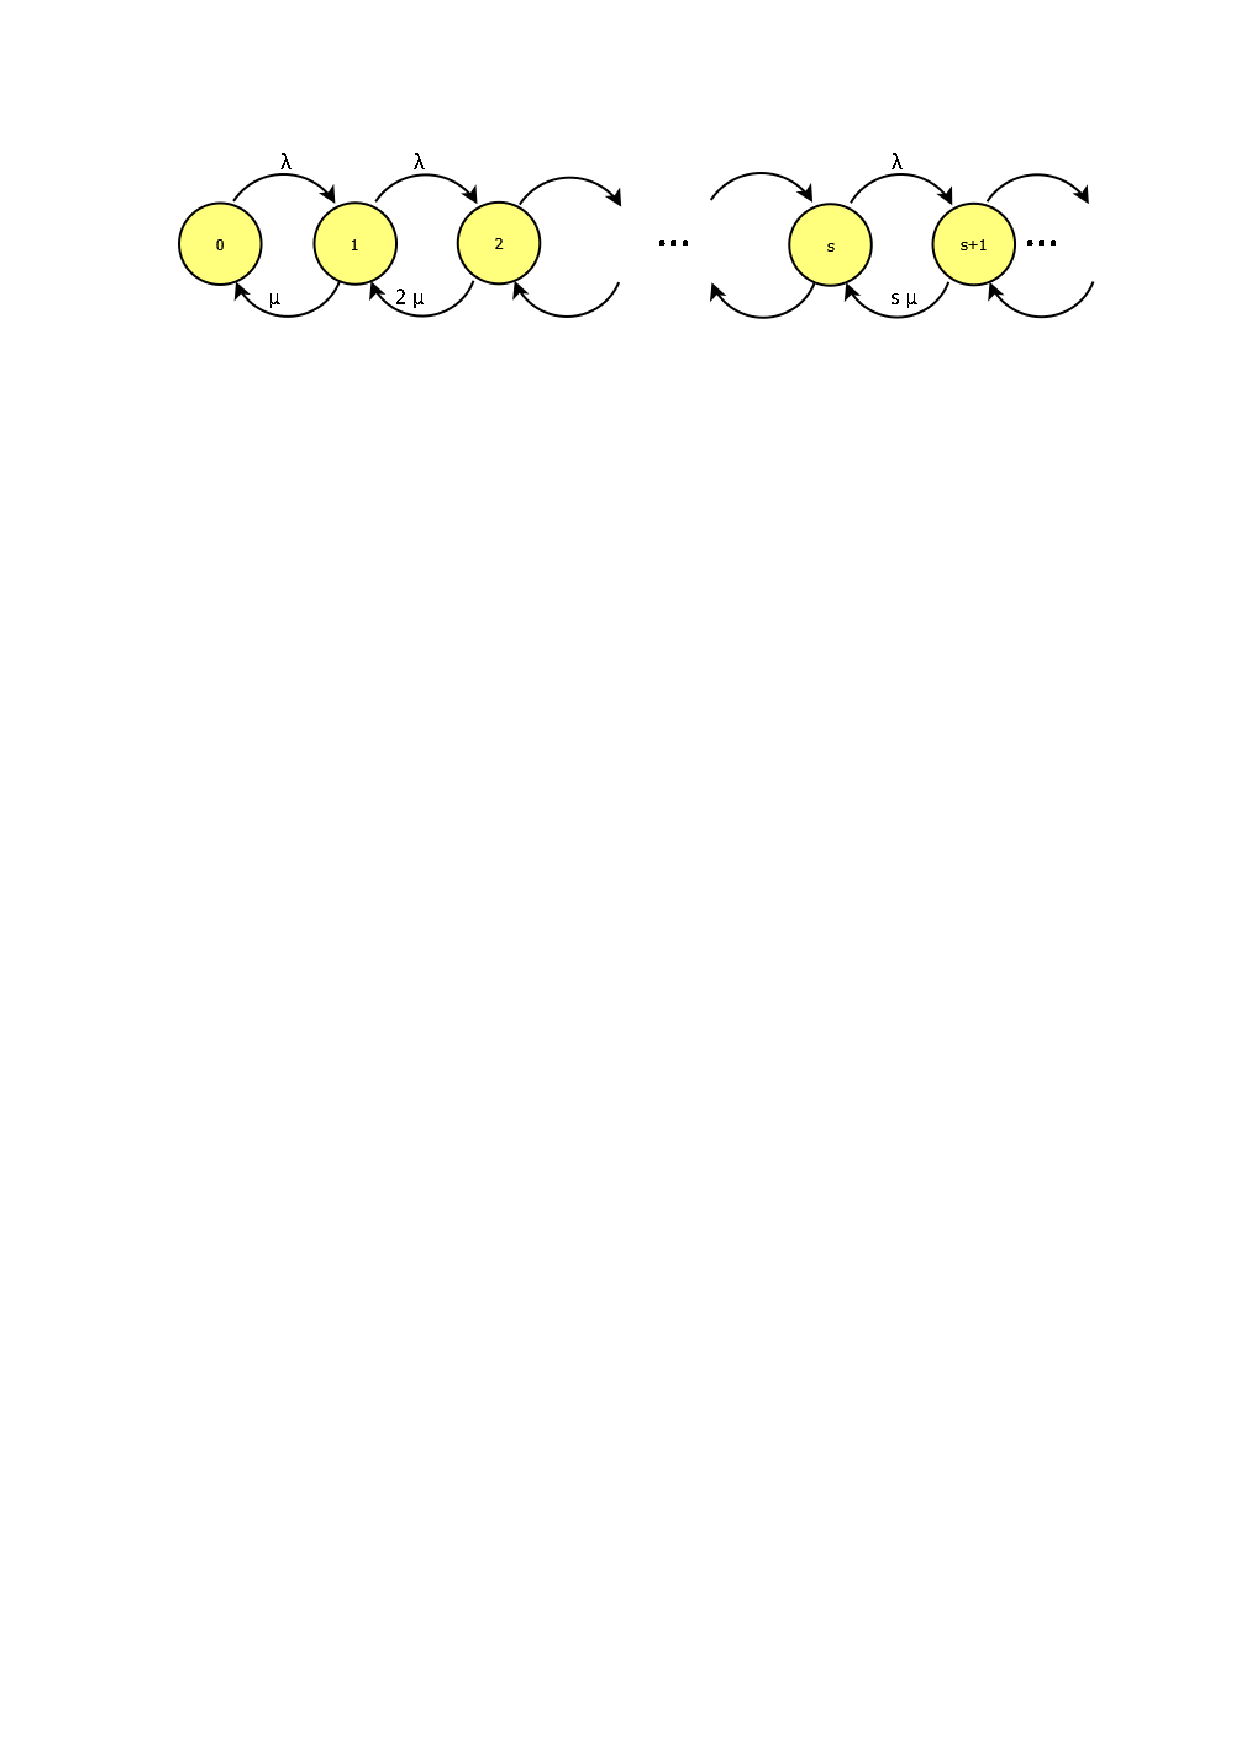
\includegraphics[trim = 10mm 220mm 10mm 25mm, clip,width=0.9\linewidth]{MMs}
		\end{figure}
		
		
		
	